\section{Modelling}
%% analyzing the real object
The object has two main parts, a cap and body. These can be constructed with simple primitives, such as cylinder and sphere. The edges of the top face of the cap and bottom face of the bottle are smooth and the base of the bottle is slightly indented as shown in figure \ref{fig:modelref}.

\begin{figure}[htbp]
    \begin{minipage}[c]{3cm}
    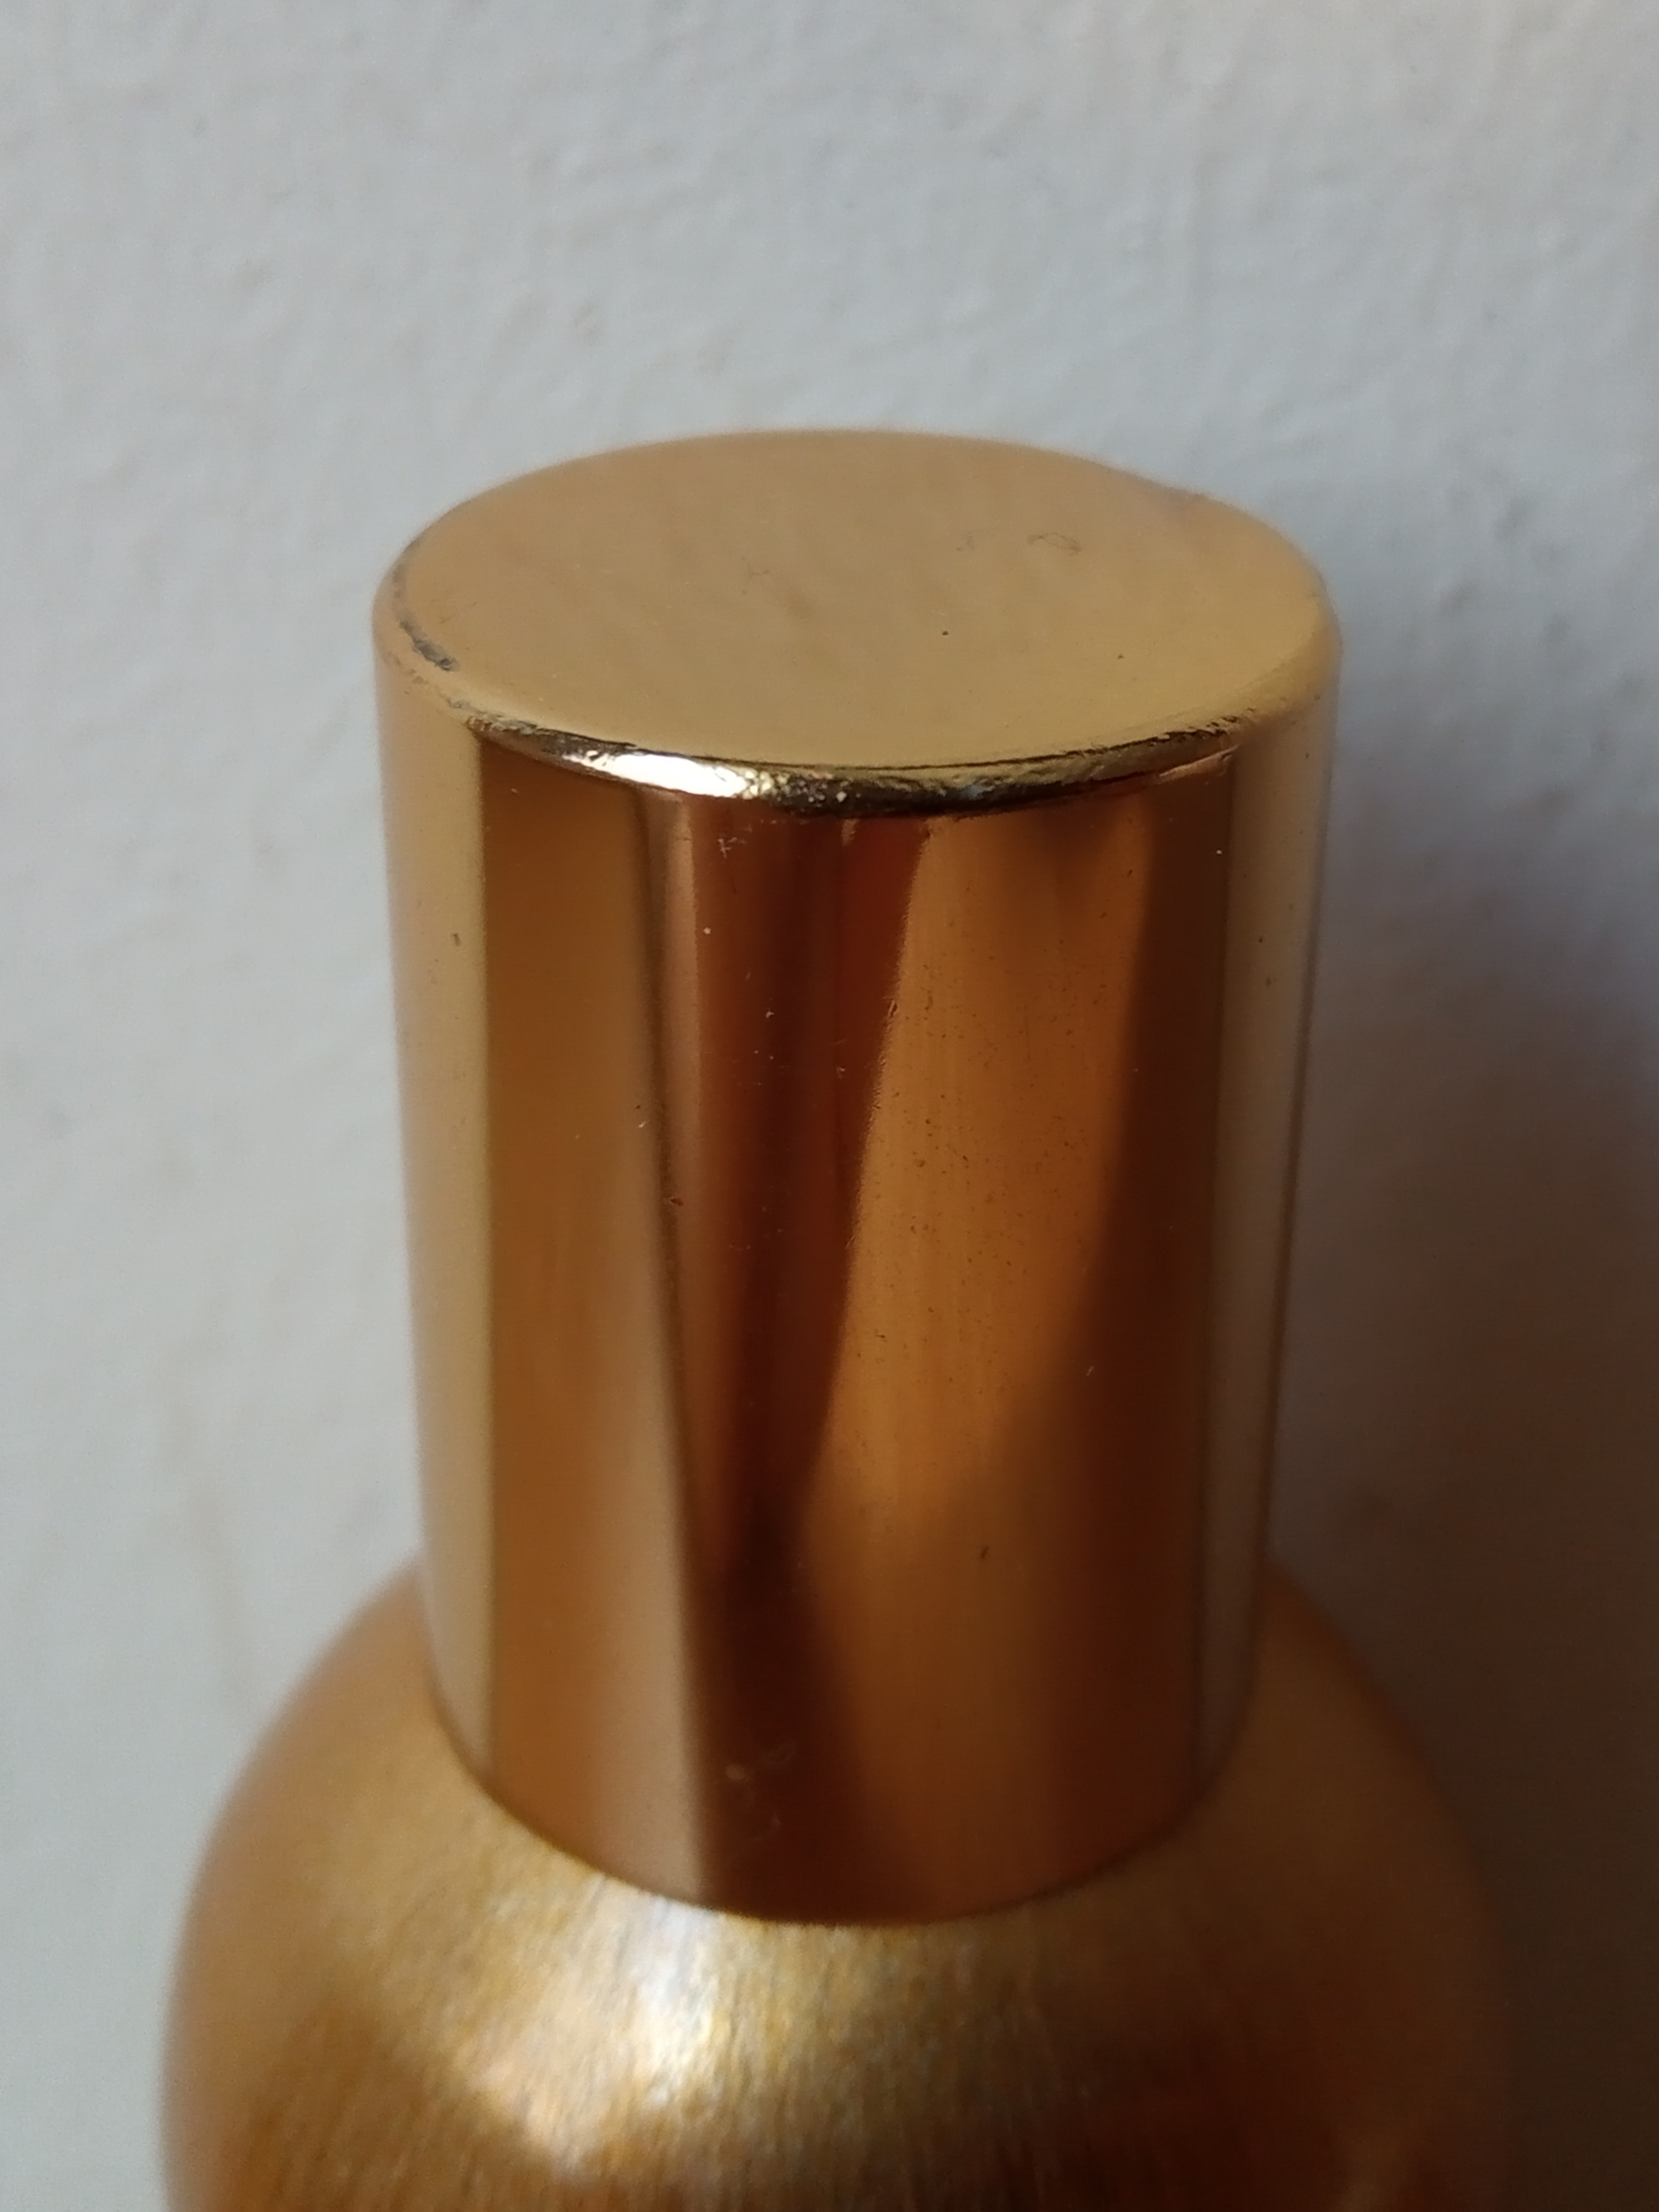
\includegraphics[width=3cm]{imgs/cap_top.jpg}
    \end{minipage}
    \begin{minipage}[c]{3cm}
        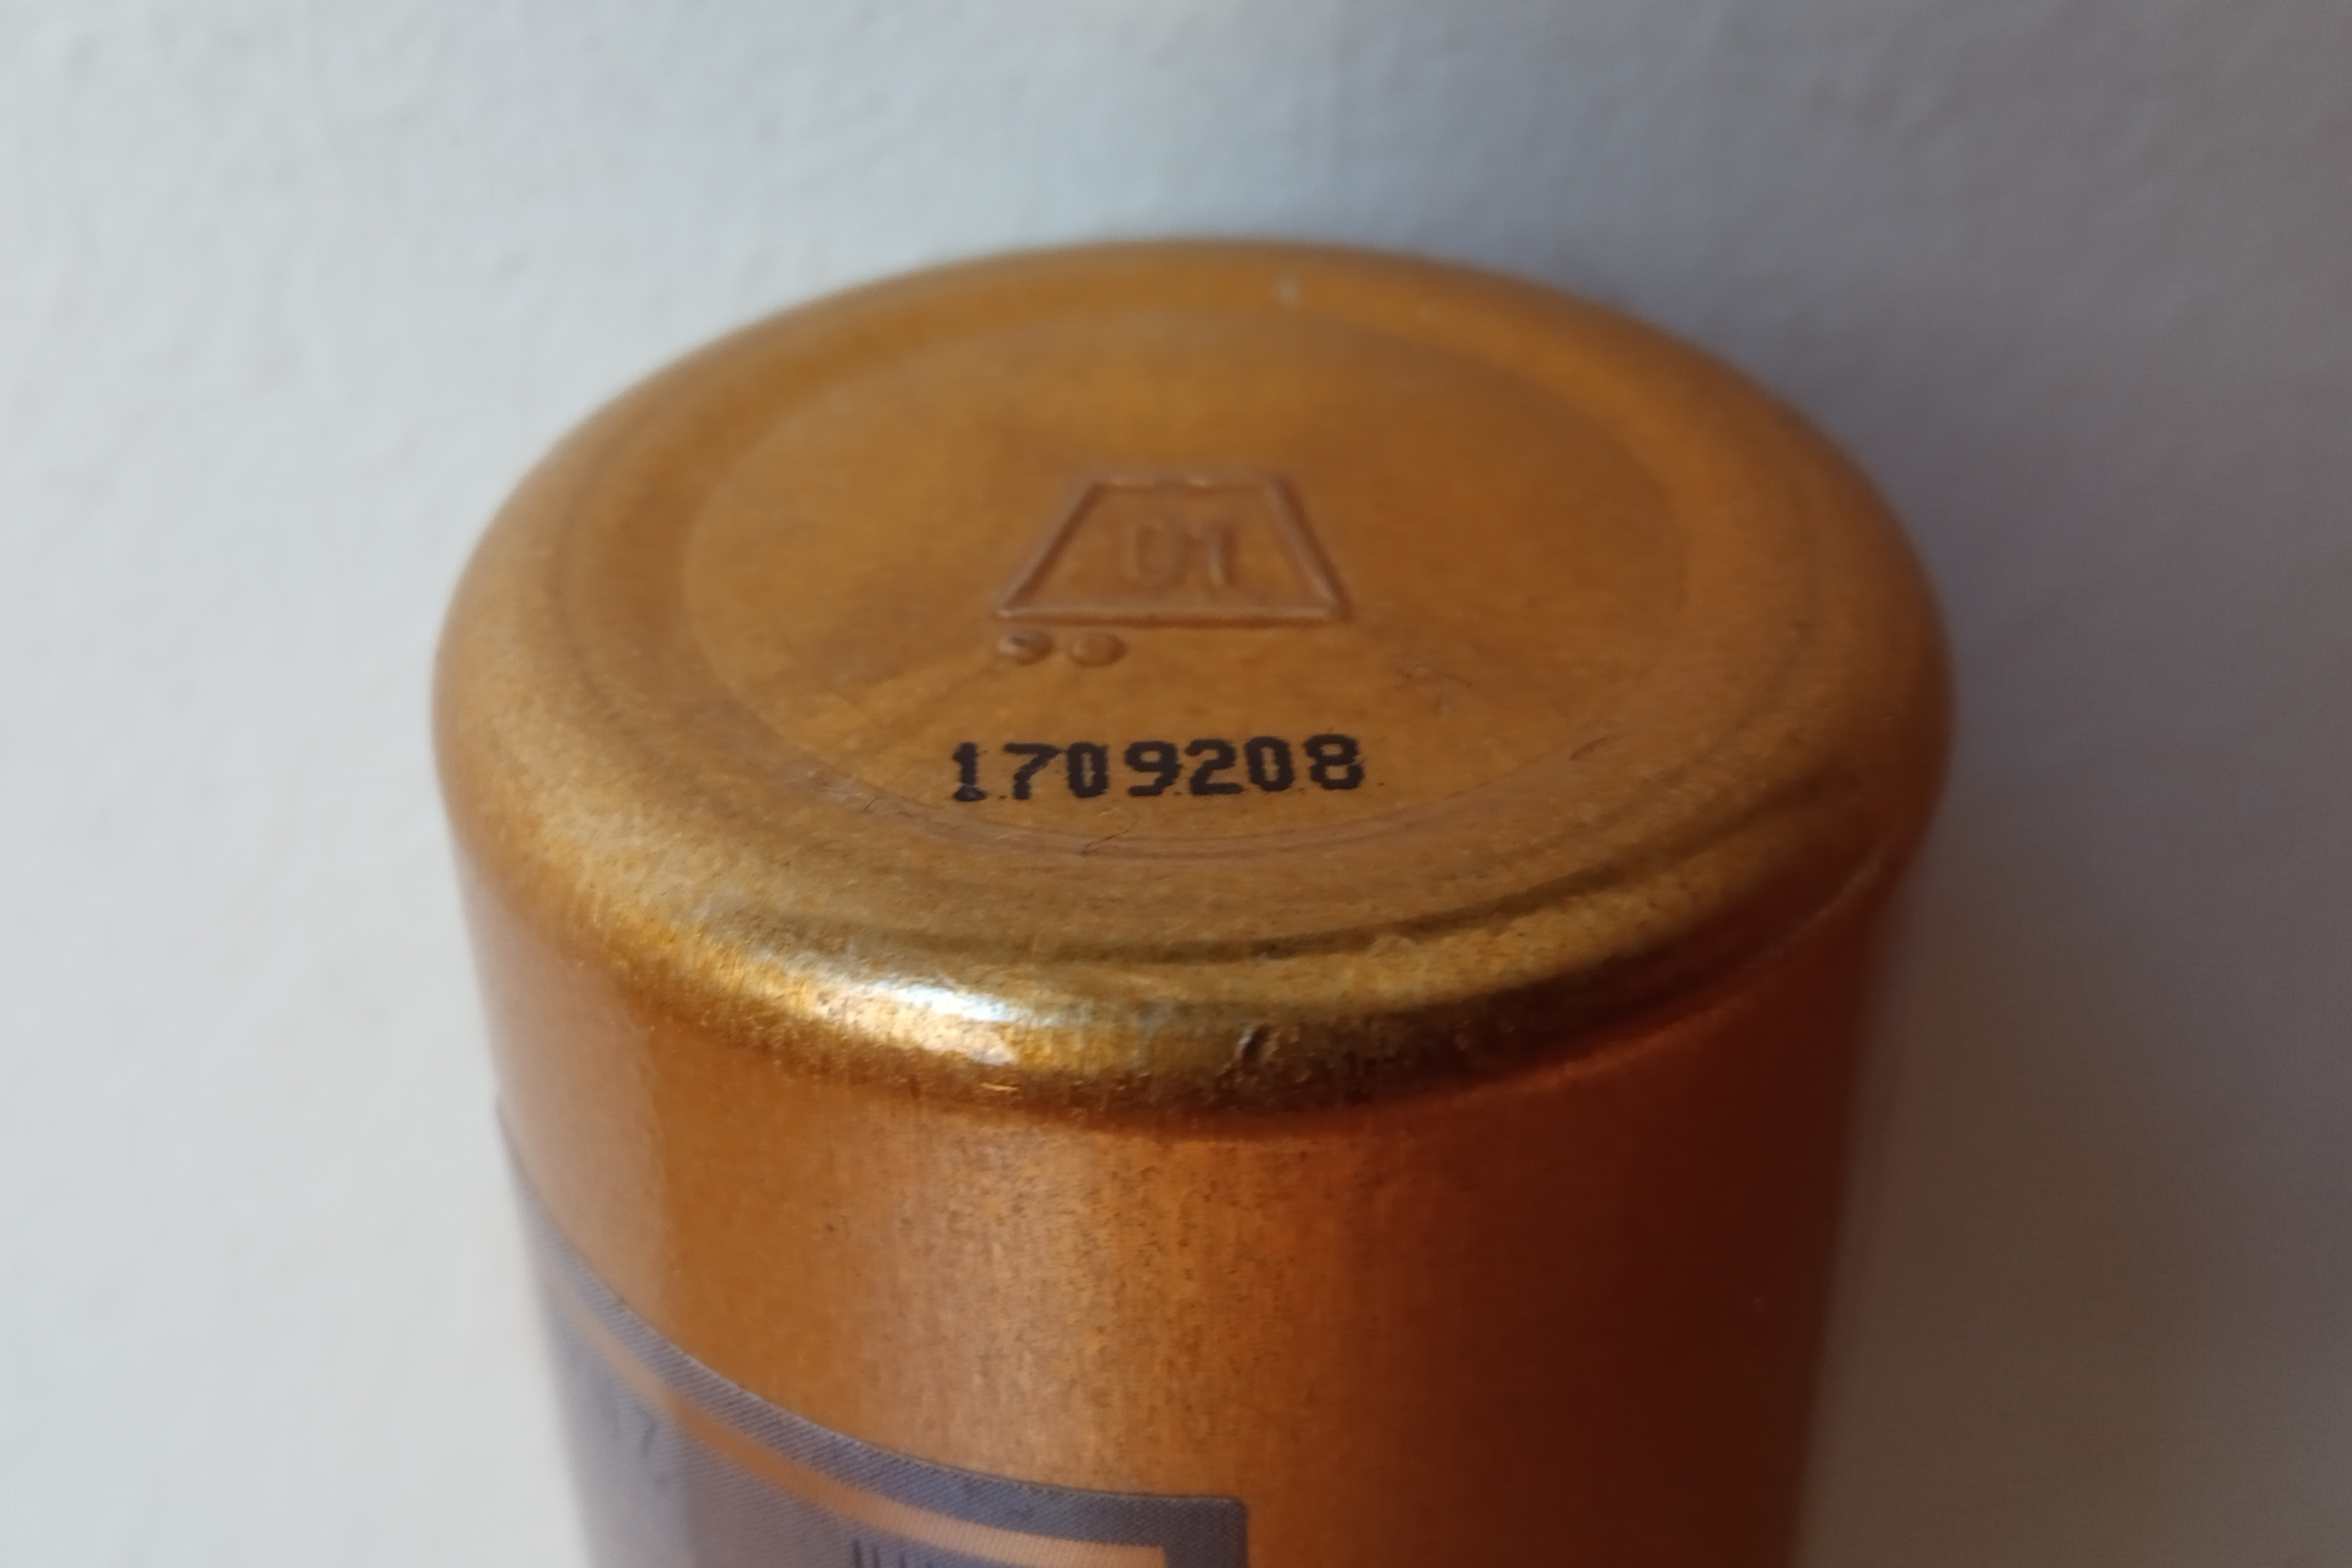
\includegraphics[width=3cm]{imgs/bottom.jpg}
        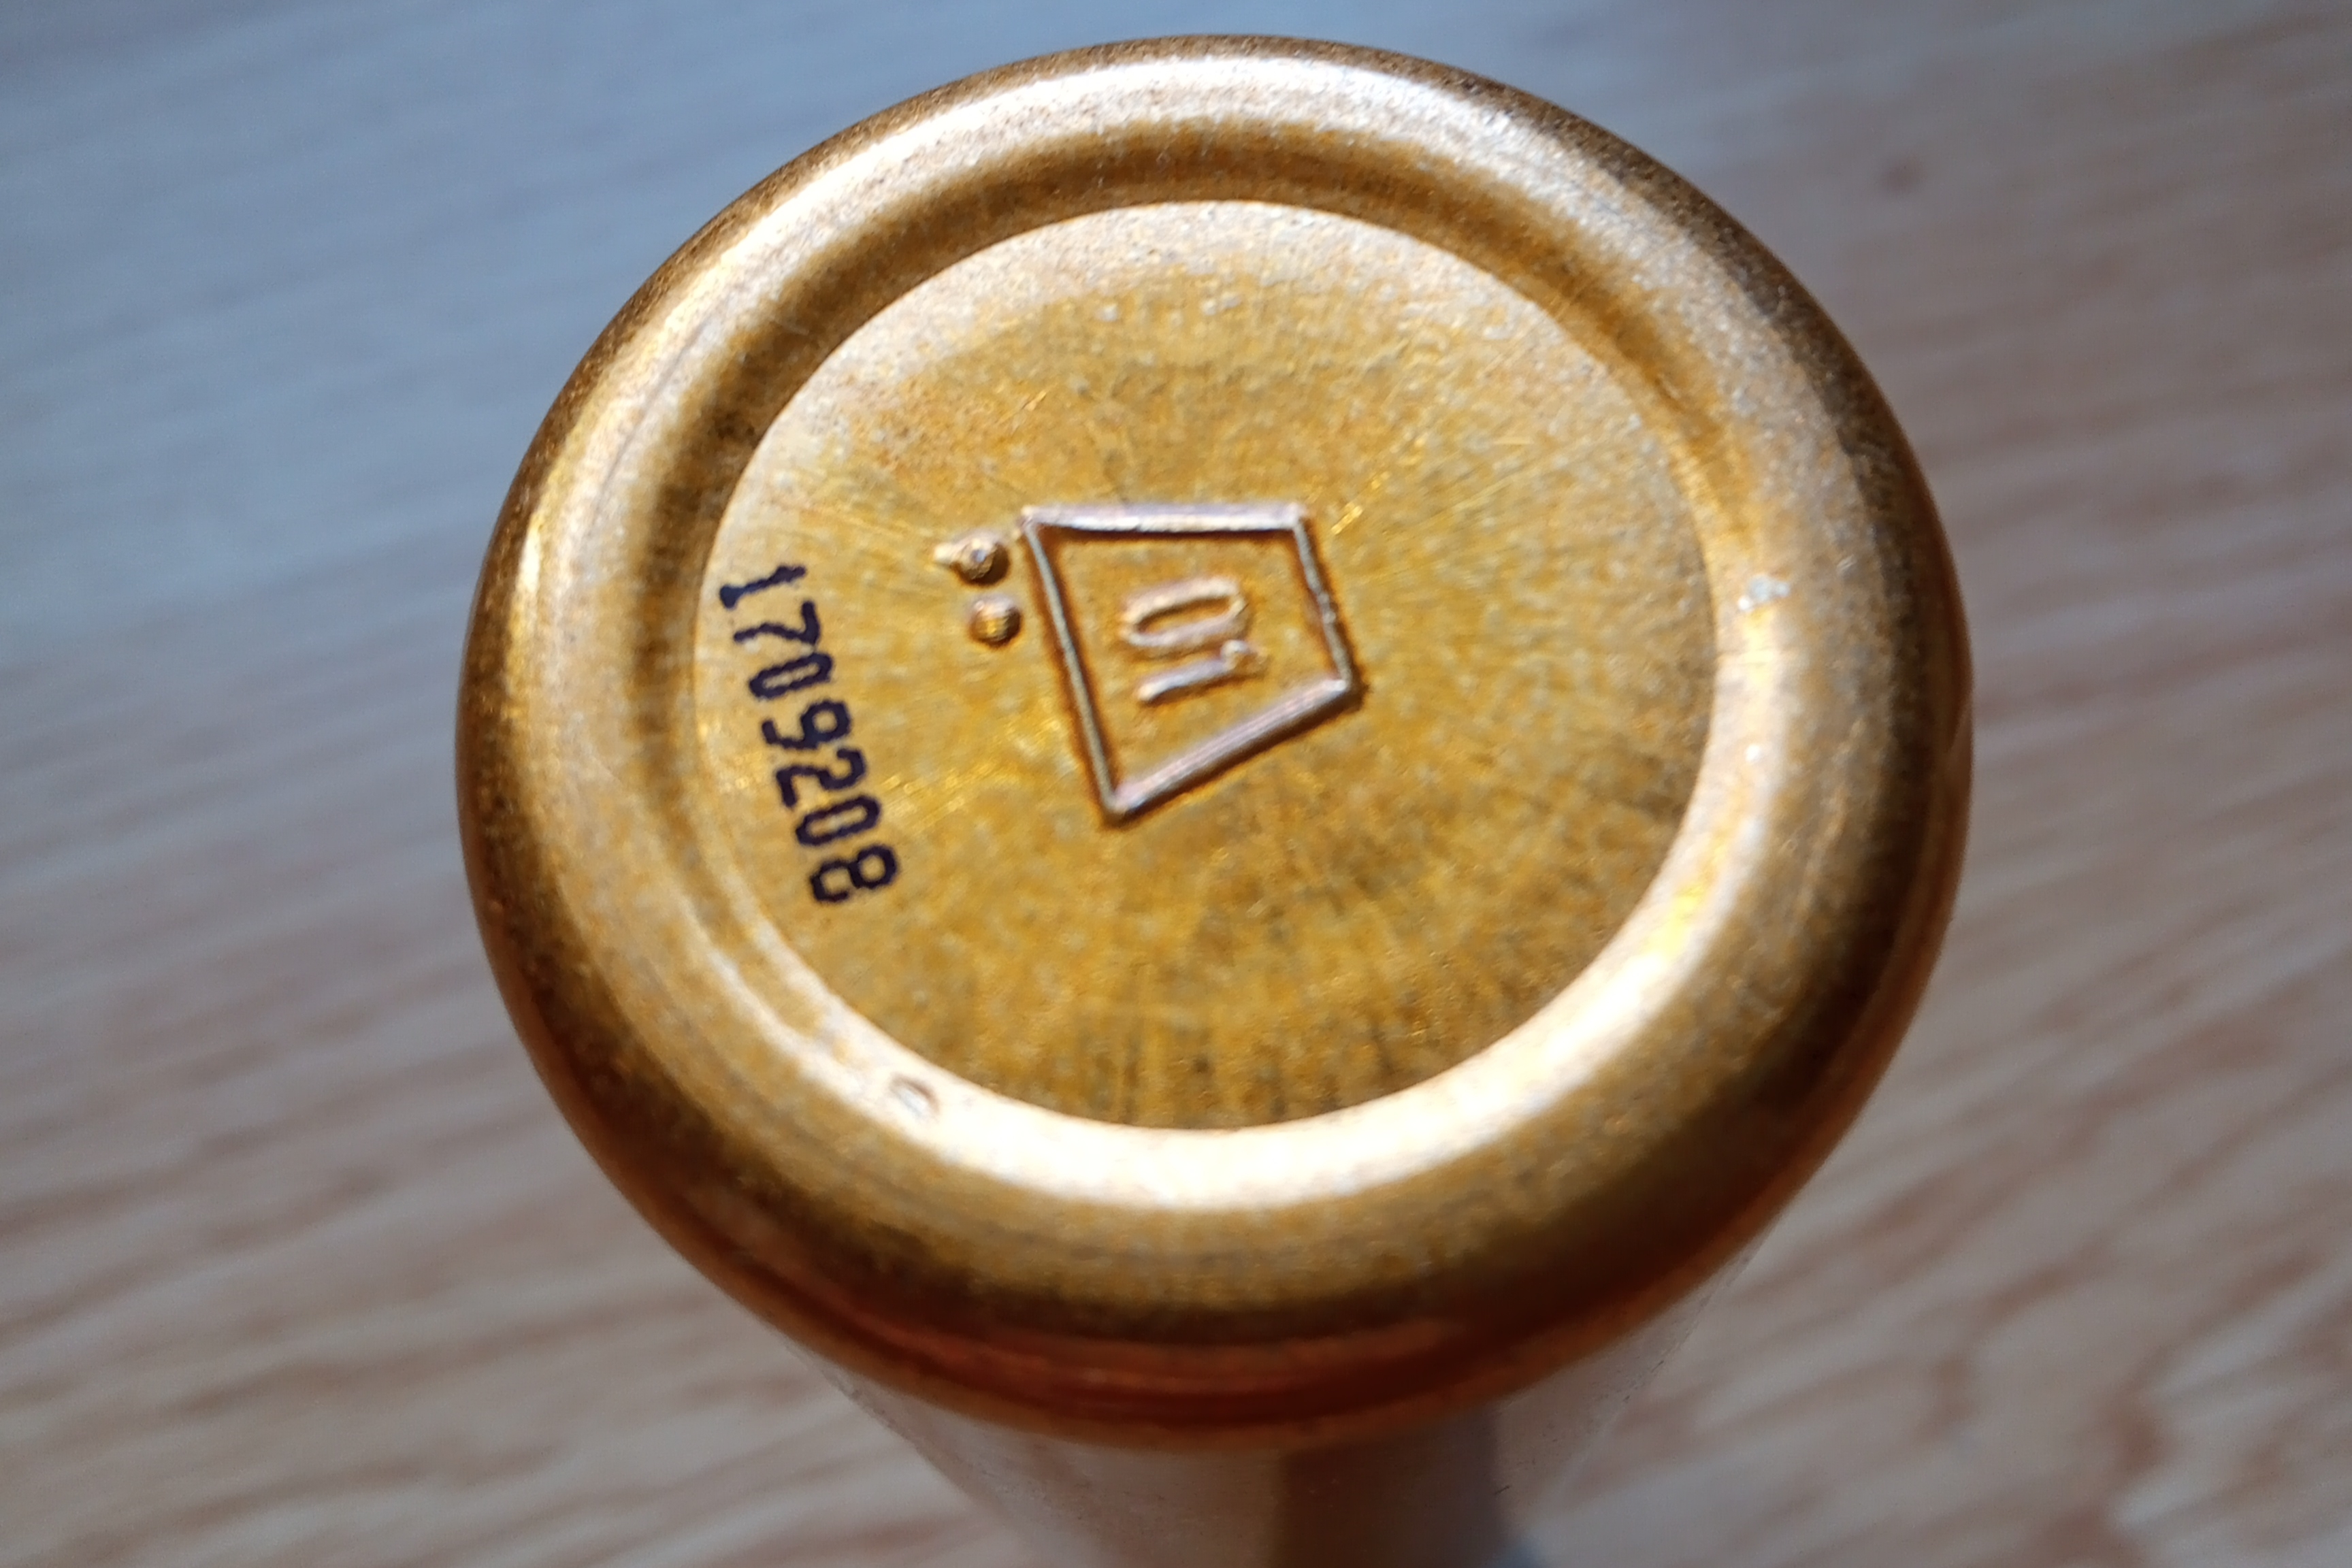
\includegraphics[width=3cm]{imgs/base.jpg}    
    \end{minipage}
    \caption{Reference images for the top of the cap (left) and the base of the bottle (right)}
    \label{fig:modelref}
\end{figure}

The object was measured to model accurately as shown in figure \ref{fig:measurement}.

\begin{figure}[htbp]
    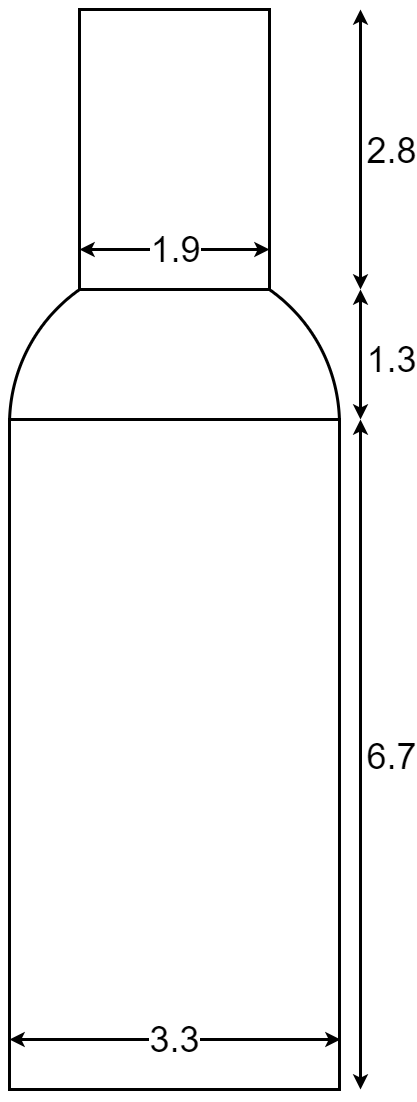
\includegraphics[height=3cm]{imgs/measurement.png}
    \hspace{1cm}
    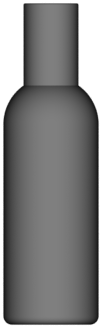
\includegraphics[height=3cm]{imgs/model_ortho.png}
    \caption{Comparison of the measurement of the real life object (left) and the modelled object in orthographic view (right)}
    \label{fig:measurement}
\end{figure}

%% describing the implementation
The object was constructed using geometric primitives with RenderMan Python API \cite{pixar2022}.
% Two cylinders for main part of body and cap.
The main part of the bottle body and the cap was constructed with cylinders.
% Sphere segment for the curved part of the body. Calculated using formulas.
The curved part of the body was reproduced by a spherical segment. The radius and the starting point of the segment was calculated with the formulas described by Weisstein \shortcite{weisstein2006}.
%%% FORMULAS

% The bottom and top using torus and disk for smooth edges.
Toruses and disks were used to construct the smooth edges at the top of the cap and the base of the bottle as shown in figure \ref{fig:model}.

\begin{figure}[htbp]
    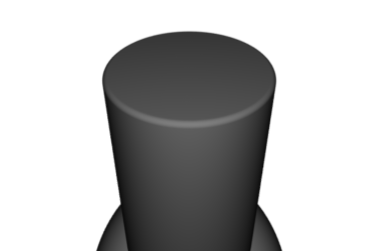
\includegraphics[width=3cm]{imgs/model_top.png}
    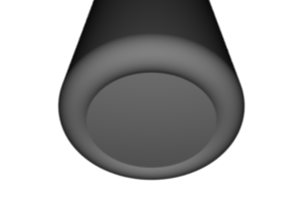
\includegraphics[width=3cm]{imgs/model_bottom.png}
    \caption{Smoothed edges of the model}
    \label{fig:model}
\end{figure}

The cap is moved slightly upwards to make a small gap between the bottle and the cap.

%%% MAYBE SHOW CALCULATION OR DIAGRAM
